%----------------------------------------------------------------------------------------
%	PACKAGES AND OTHER DOCUMENT CONFIGURATIONS
%----------------------------------------------------------------------------------------

\documentclass[
11pt, % The default document font size, options: 10pt, 11pt, 12pt
%oneside, % Two side (alternating margins) for binding by default, uncomment to switch to one side
english, % ngerman for German
singlespacing, % Single line spacing, alternatives: onehalfspacing or doublespacing
%draft, % Uncomment to enable draft mode (no pictures, no links, overfull hboxes indicated)
%nolistspacing, % If the document is onehalfspacing or doublespacing, uncomment this to set spacing in lists to single
%liststotoc, % Uncomment to add the list of figures/tables/etc to the table of contents
%toctotoc, % Uncomment to add the main table of contents to the table of contents
%parskip, % Uncomment to add space between paragraphs
%nohyperref, % Uncomment to not load the hyperref package
headsepline, % Uncomment to get a line under the header
%chapterinoneline, % Uncomment to place the chapter title next to the number on one line
%consistentlayout, % Uncomment to change the layout of the declaration, abstract and acknowledgements pages to match the default layout
]{MastersDoctoralThesis} % The class file specifying the document structure

\usepackage[utf8]{inputenc} % Required for inputting international characters
\usepackage[T1]{fontenc} % Output font encoding for international characters

\usepackage{mathpazo} % Use the Palatino font by default

\usepackage[backend=bibtex,style=authoryear,natbib=true]{biblatex} % Use the bibtex backend with the author year citation style (which resembles APA)

\addbibresource{example.bib} % The filename of the bibliography

\usepackage[autostyle=true]{csquotes} % Required to generate language-dependent quotes in the bibliography

\usepackage[breaklinks=true]{hyperref}

\usepackage{makecell}
\renewcommand\theadfont{\bfseries}

\usepackage{enumitem}

\usepackage{graphicx,wrapfig,lipsum}

\usepackage{subcaption}

\usepackage[final]{pdfpages}

%----------------------------------------------------------------------------------------
%	MARGIN SETTINGS
%----------------------------------------------------------------------------------------

\geometry{
	paper=a4paper, % Change to letterpaper for US letter
	inner=2.5cm, % Inner margin
	outer=3.8cm, % Outer margin
	bindingoffset=.5cm, % Binding offset
	top=1.5cm, % Top margin
	bottom=1.5cm, % Bottom margin
	%showframe, % Uncomment to show how the type block is set on the page
}

%----------------------------------------------------------------------------------------
%	THESIS INFORMATION
%----------------------------------------------------------------------------------------

\thesistitle{Intelligent Tree Data Management Component} % Your thesis title, this is used in the title and abstract, print it elsewhere with \ttitle
\thesistitlecz{Inteligentní komponenta pro správu stromových dat}

\supervisor{Ing. Petr \textsc{Křemen}, Ph.D.} % Your supervisor's name, this is used in the title page, print it elsewhere with \supname
\examiner{} % Your examiner's name, this is not currently used anywhere in the template, print it elsewhere with \examname
\degree{Bachlor of Software engineering and technology} % Your degree name, this is used in the title page and abstract, print it elsewhere with \degreename
\author{Jakub \textsc{Lečbych}} % Your name, this is used in the title page and abstract, print it elsewhere with \authorname
\addresses{} % Your address, this is not currently used anywhere in the template, print it elsewhere with \addressname
\keywords{Component, Filter, Linked Data, Multi-select, Select, Tree Data, Tree, React, Redux} % Keywords for your thesis, this is not currently used anywhere in the template, print it elsewhere with \keywordnames
\keywordscz{Komponenta, Třídění, Propojená data, Více násobný výběr, Výběr, Stromová data, Strom, React, Redux} %\keywordnamescz
\university{\href{https://www.cvut.cz/en}{Czech Technical University}} % Your university's name and URL, this is used in the title page and abstract, print it elsewhere with \univname
\department{\href{https://cyber.felk.cvut.cz/}{Department of Cybernetics}} % Your department's name and URL, this is used in the title page and abstract, print it elsewhere with \deptname
\group{\href{http://kbss.felk.cvut.cz}{Knowledge Based Software Systems Group}} % Your research group's name and URL, this is used in the title page, print it elsewhere with \groupname
\faculty{\href{http://www.fel.cvut.cz/en/}{Faculty of Electrical Engineering}} % Your faculty's name and URL, this is used in the title page and abstract, print it elsewhere with \facname

\AtBeginDocument{
\hypersetup{pdftitle=\ttitle} % Set the PDF's title to your title
\hypersetup{pdfauthor=\authorname} % Set the PDF's author to your name
\hypersetup{pdfkeywords=\keywordnames} % Set the PDF's keywords to your keywords
}

\newcommand\TODO[1]{\textcolor{red}{TODO:#1}}
\newcommand\CONSIDER[1]{\textcolor{blue}{CONSIDER:#1}}

\begin{document}

\frontmatter % Use roman page numbering style (i, ii, iii, iv...) for the pre-content pages

\pagestyle{plain} % Default to the plain heading style until the thesis style is called for the body content

%----------------------------------------------------------------------------------------
%	TITLE PAGE
%----------------------------------------------------------------------------------------

\begin{titlepage}
\begin{center}

\vspace*{.0\textheight}
{\scshape\LARGE \univname\par}\vspace{1cm} % University name


\includegraphics[width=.4\textwidth]{symbol_cvut_konturova_verze_cb}\vspace{1cm} % University/department logo

\textsc{\Large Bachelor Thesis}\\[0.5cm] % Thesis type

\HRule \\[0.4cm] % Horizontal line
{\huge \bfseries \ttitle\par}\vspace{0.4cm} % Thesis title
\HRule \\[1.5cm] % Horizontal line
 
\begin{minipage}[t]{0.4\textwidth}
\begin{flushleft} \large
\emph{Author:}\\
\authorname % Author name - remove the \href bracket to remove the link
\end{flushleft}
\end{minipage}
\begin{minipage}[t]{0.4\textwidth}
\begin{flushright} \large
\emph{Supervisor:} \\
\supname % Supervisor name - remove the \href bracket to remove the link  
\end{flushright}
\end{minipage}\\[3cm]
 
\large \textit{A thesis submitted in fulfillment of the requirements\\ for the degree of \degreename}\\[0.3cm] % University requirement text
\textit{in the}\\[0.4cm]
\groupname\\\deptname\\[2cm] % Research group name and department name
 
\vfill

{\large \today}\\[4cm] % Date
 
\vfill
\end{center}
\end{titlepage}

\checktoopen
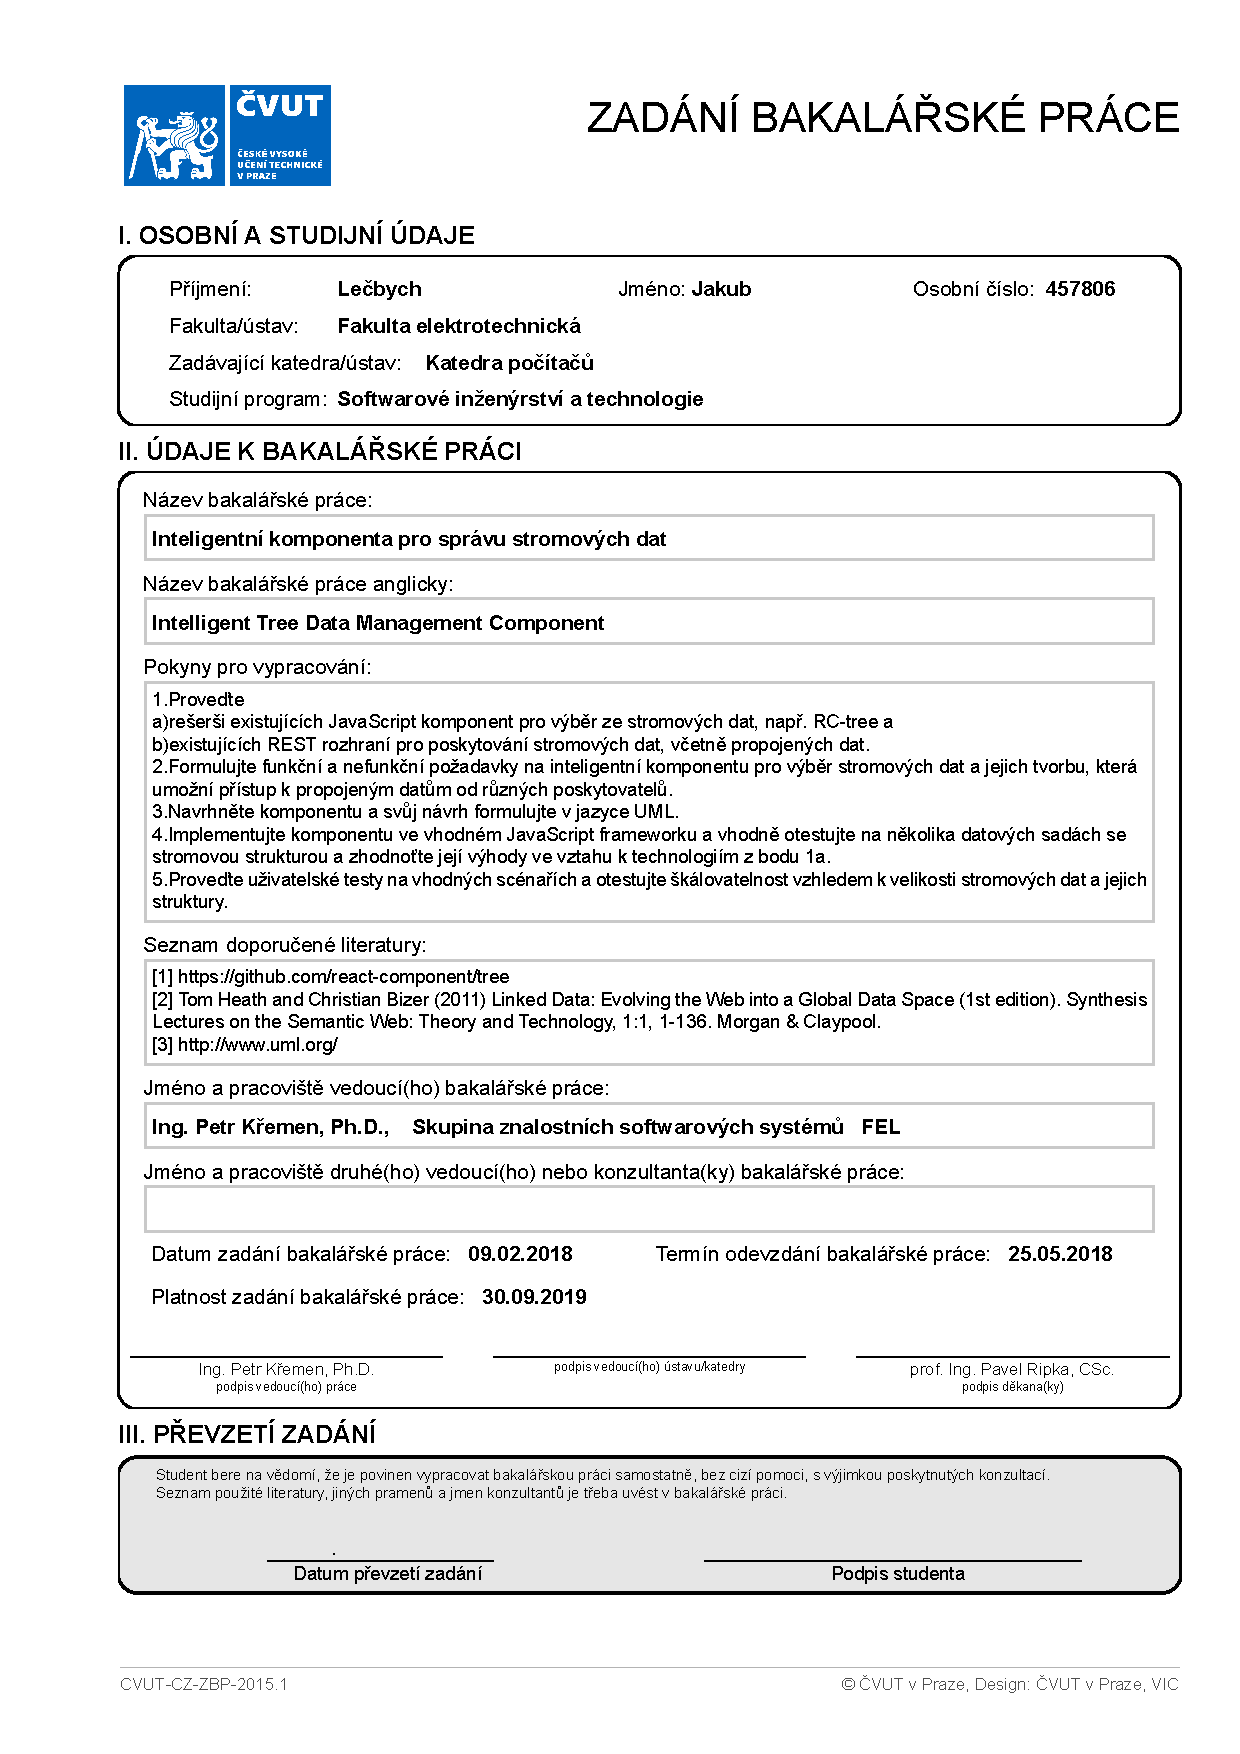
\includepdf[pages=-,pagecommand={},offset=0cm 0cm, width=1.3\textwidth]{zav_prace.pdf}


%----------------------------------------------------------------------------------------
%	DECLARATION PAGE
%----------------------------------------------------------------------------------------

\begin{declaration}
\addchaptertocentry{\authorshipname} % Add the declaration to the table of contents
\noindent I, \authorname, declare that this thesis titled, \enquote{\ttitle} and the work presented in it are my own. I confirm that:

\begin{itemize} 
\item This work was done wholly or mainly while in candidature for a research degree at this University.
\item Where any part of this thesis has previously been submitted for a degree or any other qualification at this University or any other institution, this has been clearly stated.
\item Where I have consulted the published work of others, this is always clearly attributed.
\item Where I have quoted from the work of others, the source is always given. With the exception of such quotations, this thesis is entirely my own work.
\item I have acknowledged all main sources of help.
\item Where the thesis is based on work done by myself jointly with others, I have made clear exactly what was done by others and what I have contributed myself.\\
\end{itemize}
 
\noindent Signed:\\
\rule[0.5em]{25em}{0.5pt} % This prints a line for the signature

\end{declaration}

\cleardoublepage

%----------------------------------------------------------------------------------------
%	ABSTRACT PAGE
%----------------------------------------------------------------------------------------

\begin{abstract}
\addchaptertocentry{\abstractname} % Add the abstract to the table of contents

\noindent Current UI components for working with structured tree data have some limitations. These limitations are especially performance issues when working with large datasets or support of Linked Data. After comparing and analyzing existing solutions and after the research of relevant web APIs, the design of the component is proposed, which complements these missing functions. Furthermore, this thesis describes the structure of the proposed component, its function and documents its API. Then it shows component usability and scalability in test scenarios. In conclusion, there is a summary of the results achieved and a proposal for successive steps describing the issues that need to be addressed.

\begin{abstractcz}
Současná řešení UI komponent pro práci se strukturovanými stromovými daty mají určitá omezení. Těmito omezeními jsou zejména výkonostní problémy při práci s velkými datovými objekty nebo podpora propojených dat. Po srovnání a analýze existujících řešení a následnému výzkumu relevantních webových API je navrhnuta komponenta, která doplňuje tyto chybějící funkce. Dále tato práce popisuje strukturu navrhnuté komponenty, její funkce a dokumentuje její API. Poté je ukázána její použitelnost a škálovatelnost na testovacích scénářích. Závěrem je shrnutí dosažených výsledků a návrh následných kroků, popisující problémy, které je zapotřebí vyřešit.
\end{abstractcz}

\begin{center}
{\Large\textit{Key words} \par}

\medskip
\end{center}
\noindent\keywordnames
\bigskip

\begin{center}
{\Large\textit{Klíčová slova} \par}
\medskip
\end{center}
\noindent\keywordnamescz

\end{abstract}


%----------------------------------------------------------------------------------------
%	ACKNOWLEDGEMENTS
%----------------------------------------------------------------------------------------

\begin{acknowledgements}
\addchaptertocentry{\acknowledgementname} % Add the acknowledgements to the table of contents
I would like to thanks to my supervisor \supname\ for his patience, advice, and feedback during my work on this project. Also I thanks for providing materials like example data and useful web sources to this topic.
\end{acknowledgements}

%----------------------------------------------------------------------------------------
%	LIST OF CONTENTS/FIGURES/TABLES PAGES
%----------------------------------------------------------------------------------------

\tableofcontents % Prints the main table of contents

\listoffigures % Prints the list of figures

\listoftables % Prints the list of tables

%----------------------------------------------------------------------------------------
%	ABBREVIATIONS
%----------------------------------------------------------------------------------------

\begin{abbreviations}{ll} % Include a list of abbreviations (a table of two columns)

\textbf{HTML} & \textbf{H}yper \textbf{T}ext \textbf{M}arkup \textbf{L}anguage\\
\textbf{API} & \textbf{A}pplication \textbf{P}rogram \textbf{I}interface\\
\textbf{RDF} & \textbf{R}esource \textbf{D}escription \textbf{F}ramework\\
\textbf{IRI} & \textbf{I}nternationalized \textbf{R}esource \textbf{I}dentifier\\
\textbf{URI} & \textbf{U}niform \textbf{R}esource \textbf{I}dentifier\\
\textbf{JSON} & \textbf{J}ava\textbf{S}cript \textbf{O}bject \textbf{N}otation\\

\end{abbreviations}

%----------------------------------------------------------------------------------------
%	THESIS CONTENT - CHAPTERS
%----------------------------------------------------------------------------------------

\mainmatter % Begin numeric (1,2,3...) page numbering

\pagestyle{thesis} % Return the page headers back to the "thesis" style

% Include the chapters of the thesis as separate files from the Chapters folder

% Chapter Template

\chapter{Introduction} % Main chapter title

\label{Chapter1} % For referencing the chapter elsewhere, use \ref{Chapter1} 

%----------------------------------------------------------------------------------------
%	SECTION 1
%----------------------------------------------------------------------------------------

\section{Overview}

Data, pieces of information that are measured, collected, analyzed and used for different kinds of things. Such data are distinguished based on their structure - unstructured (e.g., a list of strings) or structured (e.g., a graph), on their type - specific or general, and so on. Structured data are often represented as a graph. Human intuition allows us to understand these graph connections with no problem, but computers do not have that intuition. So the data context must be defined to enable the computer to understand these connections between the data and the meaning of that data. This problem is one of the main reasons why people created a concept of the Web Ontology Language \parencite{OWL}. However, more about that will be down below.


Data are in many cases provided through the web APIs. The most straightforward definition of the web APIs is following.
Web API is the interface through which an application can communicate with that server. Then fragmentation of the web APIs is so significant that many existing solutions support only one type
and does not allow to get responses from multiple APIs simultaneously. More detailed
information about web API is in Chapter 3.


With all that data provided by the web APIs, there is a question - “How to render that data as options efficiently?”.  Because rendering large lists, is operation can be time-consuming and can affect the performance of an application significantly. Performance is one of the most critical aspects of the modern applications. Based on the study \parencite{Tolarance_study} the delay of 2 seconds is the limit where a response to simple commands becomes unacceptable to users.

%----------------------------------------------------------------------------------------
%	SECTION 2
%----------------------------------------------------------------------------------------

\section{Current situation}

UI developers often need to use a tree select input in their applications. The Problem is that default HTML select input is not usable in many cases. Also, most current solutions cannot handle complex data (e.g., graph data) or cannot render large data lists efficiently. Moreover, if the developers finally find a solution with functionality that they need, the solution does not fit by design into their application. So in many cases, they have to develop their component for that specific problem.


%----------------------------------------------------------------------------------------
%	SECTION 3
%----------------------------------------------------------------------------------------

\section{Thesis goal}

The primary goal of this bachelor thesis was to create a UI component that will support all features of the previous component such as rendering data as a tree, support of linked data, and support of graph type data structure. Also, the component should provide several new features. These features are:
\begin{itemize}
\item selecting or multi-selecting options
\item simplicity of use and integration with other applications
\item flexibility (e.g. customization, different types of datasets)
\item re-usability
\item good performance with large datasets
\item creating new options
\end{itemize}


%----------------------------------------------------------------------------------------
%	SECTION 4
%----------------------------------------------------------------------------------------

\section{Outline}

This thesis is divided into two main parts - research part and implementation part. In the research part, the primary focus will be on the technology and work related to this problem. The second part will describe the implementation of the component, logical structure, and behavior. So the second chapter will be dedicated to the used technology, and to the related problems. Especially the Linked Data and the concept of the semantic web. Then we will have a look at the APIs that provide these data, their construction and how they behave. In the next part, we will look at the technical aspects of the component such. Then the focus will be on the component itself. A chapter about implementation will describe individual parts or sub-components and at the end of that chapter algorithms for filtering and rendering will be described. In the end, there will be a comparison of other solutions and benchmark. The last chapter will summarise the results and describe future steps.


%----------------------------------------------------------------------------------------
%	SECTION 5
%----------------------------------------------------------------------------------------

\section{Term definition}

In this theses will be often used a several terms. To avoid any misunderstanding this table shows description of each term.

\begin{center}
    \begin{longtable}{ | l | p{10cm} | }
    \caption{Definition of terms used in this thesis} \label{tab:definition} \\
    \hline 
    \multicolumn{1}{|c|}{\textbf{Term}} & 
    \multicolumn{1}{c|}{\textbf{Description}}
	\endfirsthead
    
    \hline 
    select input & HTML element represented as <input type='select'/> \\ \hline
    dropdown menu & HTML elements displayed under select input. This element contains individual options \\ \hline
    option & Part of the dropdown men. Option represent one data object. Example of data object: \{value: '123', label: 'option label'\} . \\ \hline
    option provider & Web API providing data. \\ \hline
    search & Process of filtering and rendering results of filter subprocess in form of dropdown menu with options. \\ \hline
    \end{longtable}
\end{center}

%----------------------------------------------------------------------------------------
% Chapter Template

\chapter{Background} % Main chapter title

\label{Chapter2} % For referencing the chapter elsewhere, use \ref{Chapter1} 

One of the requirements of this thesis was the ability to work with linked data. As well as the React framework, because of high usage of that framework in other projects that are developed by \groupname. So now in this chapter, introduce the technologies that are related to this thesis.

%----------------------------------------------------------------------------------------
%	SECTION 1
%----------------------------------------------------------------------------------------

\section{Resource Description Framework}

Resource Description Framework \parencite{Guha+Brickey+McBride} is a general description framework for describing informations provided by web sources. This framework creates a basis for the semantic web. Representation of the RDF can be as a graph or dataset. 

In graph representation, data are a set of RDF triplets. Each triplet consists of three components - subject, predicate, and object. Subject and object are nodes and predicate is an edge of the graph. Triplet in official terminology express some facts about the source. A claim consists of three pieces that together create a sentence: subject --> predicate --> object.  Within this statement, the source is a subject identified by URI (or IRI), the property is a predicate (what we say about the source), and value is an object. Predicates that we used for describing a source come from so-called schemas – that are
vocabularies or ontologies. Examples can be \cite{DC} or \cite{foaf} metadata standards. RDF syntax has various type of formats that are called serialization formats. Among these formats are for example Turtle, N-Quads, N-Triplets, or JSON-LD.\parencite{JSON-LD}

An RDF dataset is a set of RDF graphs. This set can consist of:
\begin{itemize}
\item default graph - exactly one RDF graph that does not have a name and may be empty
\item named graphs - a pair of RDF graph and IRI or blank node
\end{itemize}


%----------------------------------------------------------------------------------------
%	SECTION 2
%----------------------------------------------------------------------------------------

\section{Linked Data}

To understand what is Linked Data, you do not need any experience with web programming, just a basic knowledge of HTTP, URI, and IRI. The concept of Linked Data \parencite{Bizare+heath+Berners-Lee,Heath+Bizer} is following. Firstly, lest start what data are. Data are sets of values consisting of pieces of information. Problem with these data is that they do not carry any context about the information they represent. Imagine this example, two different data objects both objects have a property called 'name' with some value. That property represents some name, but without any further knowledge, that name representation can have a different meaning in each object.

On the other hand, Linked Data help to solve the problem by describing and interconnecting data by shared vocabularies. By packaging a data in the way that they express what kind of data they represent,  you will receive a Linked Data. With all of this, there are still two main problems. First is what format use for Linked Data. There are lots of formats, for example, JSON, RDFa, XML, CSV, HTML, etc. The second problem is how we can link the pieces of data together. Most common and easiest way to express data is on the key-value pair. 

%----------------------------------------------------------------------------------------
%	SECTION 3
%----------------------------------------------------------------------------------------

\section{JSON-LD}
JSON-LD is a format based on JSON format. JSON format is easy to use in a web application because it is readily convertible to JavaScript object, which represents data in a web application


JSON-LD is an RDF syntax for describing linked data using JSON format. \parencite{JSON-LD} JSON-LD is both JSON document and RDF document \parencite{RDF_doc}, but it has some differences with RDF. First, JSON-LD properties can be URIs (or IRIs) or blank nodes whereas in RDF properties must be URIs (or IRIs). That means that JSON-LD can serialize RDF data-sets. The other direction is not possible. Second, JSON-LD object lists are part of data model whereas RDF objects are part of the vocabulary. The last one, RDF values are either literals or language-tagged strings whereas JSON-LD also supports JavaScript native types, which are numbers, booleans, and strings.

\begin{figure}[th]
    \centering
    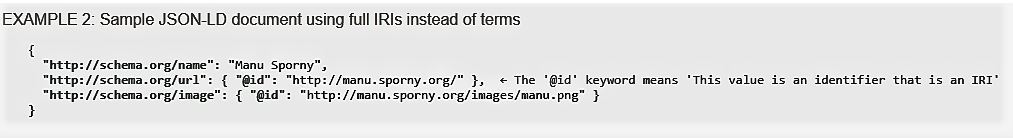
\includegraphics[width=\textwidth]{JSON-LD_example}
    \decoRule
    \caption[JSON-LD document]{Example of JSON-LD document}
    \label{fig:JSON-LD_document}
 \end{figure}

%----------------------------------------------------------------------------------------
%	SECTION 4
%----------------------------------------------------------------------------------------

\section{React, Redux}

React \parencite{react} is a JavaScript UI framework developed and maintained by Facebook. Its one of the most used framework because it's easy to learn and because of its performance efficiency. If
you are familiar with the MVC model\parencite{MVC}, React is only the view part. Redux \parencite{Redux} is completely independent on React. Redux is a state container for JavaScript. This means, that Redux is just a framework for managing the state of your web applications. It evolves from Flux \parencite{Flux} framework but does not take Flux complexity.

%----------------------------------------------------------------------------------------
%	SECTION 5
%----------------------------------------------------------------------------------------

\section{React virtualized select and React select}

\cite{react-virtualized-select} and \cite{react-select} as the name suggests, are both
React components. Both components are almost same.  As the Brian Vaughn says: 
"react-select-virtualized works just like react-select". The only difference between them 
is that the first component is able to render large list more efficiently. This was 
achieved by a special way of rendering options. In a nutshell, the drop-down menu is 
rendered only with a minimum required amount of options that are in focus (visible in 
the drop-down menu). A detailed description of this process will be described later on.

%---------------------------------------------------------------------------------------- 
% Chapter Template

\chapter{Related work} % Main chapter title
\label{Chapter3} % Change X to a consecutive number; for referencing this chapter elsewhere, use \ref{ChapterX}


In this chapter, I will compare three existing solutions. I choose these three solutions because they are the solutions with the highest number of downloads (more than 5000 per month. In case of rc-tree select 270 thousand per month). Also, all three solutions have most of their functionality similar or same to mine. These similar features are:
\begin{itemize}
\item selecting/ multi-selecting options
\item displaying data as a tree or as a list
\item toggle/ expand function for each option with children options
\item filtering/ highlighting results
\end{itemize}

So I will not compare these functionalities, only the benefits, and disadvantages of each solution.

%----------------------------------------------------------------------------------------
%    SECTION 1
%----------------------------------------------------------------------------------------

\section{React dropdown tree select}

One of the alternatives to my work is React dropdown tree select \parencite{react-dropdown-tree-select}.
  
\begin{center}
    \begin{longtable}{|p{7cm}|p{7cm}|}
      \hline 
      \multicolumn{1}{|c|}{\textbf{Pros}} & 
      \multicolumn{1}{c|}{\textbf{Cons}}
      \endfirsthead
      
      \multicolumn{2}{c}%
	{\tablename\ \thetable\ -- \textit{Continued from previous page}} \\
	\hline
	\multicolumn{1}{|c|}{\textbf{Pros}} & \multicolumn{1}{c|}{\textbf{Cons}} \\
    \endhead
    \multicolumn{2}{r}{\textit{Continued on next page}} \\
	\endfoot
    \hline
	\endlastfoot
    \hline
    
        Design can be overridden to match Bootstrap \parencite{bootstrap} or Material design \parencite{material_design} frameworks.
        & All nodes are collapsed by default and cannot be expanded altogether. \\
        \hline
        Search debouncing - The tree debounces key presses to avoid costly search calculations. The default duration is 100ms. 
        & Cannot collapse/ uncollapse tree nodes during a search. \\
        \hline
        & Component does not support highlighting of matched text during a search. \\
        \hline
        & Component does not support asynchronous data loading. \\
        \hline
        & Data must have label and value properties. \\
        \hline
        & Data cannot be represented as an array of graph nodes.  Parent node must have child property to display children nodes and so on. This main problem with this approach is that for manipulating with some node, you need whole tree branch. Also, it is hard to calculate the length (total number of options) in this data structure. \\
        \hline
        & Renders all relevant options at once, this can slow performance of the component. \\
        \hline
    \end{longtable}
\end{center}

%----------------------------------------------------------------------------------------
%    SECTION 2
%----------------------------------------------------------------------------------------

\section{RC tree select}

First competitive solution is a React tree select component \parencite{rc-tree}. However, as I found out this solution is just a React solution of Ant design component. Moreover, nowadays Ant design components work with React as well so I do not see a point to use this component.

\begin{center}
    \begin{longtable}{|p{7cm}|p{7cm}|}
      \hline 
      \multicolumn{1}{|c|}{\textbf{Pros}} & 
      \multicolumn{1}{c|}{\textbf{Cons}}
      \endfirsthead
      \multicolumn{2}{c}%
	{\tablename\ \thetable\ -- \textit{Continued from previous page}} \\
	\hline
	\multicolumn{1}{|c|}{\textbf{Pros}} & \multicolumn{1}{c|}{\textbf{Cons}} \\
    \endhead
    \multicolumn{2}{r}{\textit{Continued on next page}} \\
	\endfoot
    \hline
	\endlastfoot
    \hline
      & Does not support highlighting of matched text during search. \\
      \hline
      & Selected items can be removed only via checkboxes. Other solutions have small '$\times$' button that can remove corresponding option. But in the case of this solution you need at least two steps to remove a selected option. (1. find that option 2. uncheck it) \\
      \hline
      & Renders all relevant options at once which can slow performance of the component. \\
      \hline
    \end{longtable}
\end{center}


%----------------------------------------------------------------------------------------
%    SECTION 3
%----------------------------------------------------------------------------------------
\pagebreak

\section{Ant design tree select}

Last one is a tree select from Ant design \parencite{Ant.Design}. 

\begin{center}
    \begin{longtable}{|p{7cm}|p{7cm}|}
      \hline 
      \multicolumn{1}{|c|}{\textbf{Pros}} & 
      \multicolumn{1}{c|}{\textbf{Cons}}
      \endfirsthead
      \multicolumn{2}{c}%
	{\tablename\ \thetable\ -- \textit{Continued from previous page}} \\
	\hline
	\multicolumn{1}{|c|}{\textbf{Pros}} & \multicolumn{1}{c|}{\textbf{Cons}} \\
    \endhead
    \multicolumn{2}{r}{\textit{Continued on next page}} \\
	\endfoot
    \hline
	\endlastfoot
    \hline
      Complete ecosystem with other Ant design components.
      & Render all relevant options at once this can slow performance of the component. \\
      \hline
      Maintained and updated on a regular basis by the Ant UED team.
      & Does not cashed previous search result. For every new character (searched string)
      they filter through original data set. \\
      \hline
      Solutions for other UI frameworks like Angular, Vue, Ember and ClojureScript
      & \\
      \hline
    \end{longtable}
\end{center}

  
%----------------------------------------------------------------------------------------
%    SECTION 4
%----------------------------------------------------------------------------------------

\section{Summary of the related works}

Each of these solutions provides expected functionality from this type of component. Also, these component are popular to use, that supports a fact of the high download rate. On the other hand, none of these components is useful for rendering a large number of options. Moreover, none provide the functionality of Intelligent tree select component such as support of multiple data providers.

%----------------------------------------------------------------------------------------
% Chapter Template

\chapter{Design} % Main chapter title

\label{Chapter4} % Change X to a consecutive number; for referencing this chapter elsewhere, use \ref{ChapterX}

 
%----------------------------------------------------------------------------------------
%	SECTION 1
%----------------------------------------------------------------------------------------

\section{Requirements}

Requirements are distinguished into the two categories, functional, and non-functional. Each category has requirements specified for the user, and for a developer. A user is a person that use or communicate with the component in the form of actions like searching or filtering. Requirements are defined based on the assignment as well as based on the functionalities of the current solutions.

%----------------------------------------------------------------------------------------
%	SUBSECTION 1.1
%----------------------------------------------------------------------------------------

\subsection{Functional}

Functional requirements related to the user are following:
\begin{enumerate}
    \item Component must support multiple options providers
    \item Dropdown with results will be displayed on focus
    \item Each option should show its state (additional info such as - comment, providers, or its state)
    \item User must be able to filter among these options
    \item Selection and multi-selection must be provided
    \item The component must provide a way to create new options
    \item The component should accept and visualize tree-structured data.
\end{enumerate}
Other functional requirements for developers
\begin{enumerate}[resume]
    \item The component must be able to work with linked data sources
    \item The component should support multiple input formats – JSON (because of the easy interpretation on the client side) and XML (because of the wide marketplace) 
\end{enumerate}

%----------------------------------------------------------------------------------------
%	SUBSECTION 1.2
%----------------------------------------------------------------------------------------

\subsection{Non-Functional}

Non-functional requirements
\begin{enumerate}
    \item Operations like search and render must be scalable without negative impact on the user experience
    \item Processing data, filtering and rendering should be real-time (not take longer than acceptable)
\end{enumerate}
Other non-functional requirements for developers
\begin{enumerate}[resume]
    \item Component must be easily integrable with React applications
    \item Component must be flexible – custom styling, own filter method and render method
\end{enumerate}

%----------------------------------------------------------------------------------------
%	SECTION 2
%----------------------------------------------------------------------------------------

\section{Use-cases}
 
Based on the requirements, I identified the following use-cases. There are two actors, a developer and a user of the component. The focus of the use cases for the user is mainly on the interaction between user and data displayed by the component in the form of options. On the other hand for the developer use-cases are focused on the needs to integrate the component into their applications.
 
 \begin{figure}[th]
    \centering
    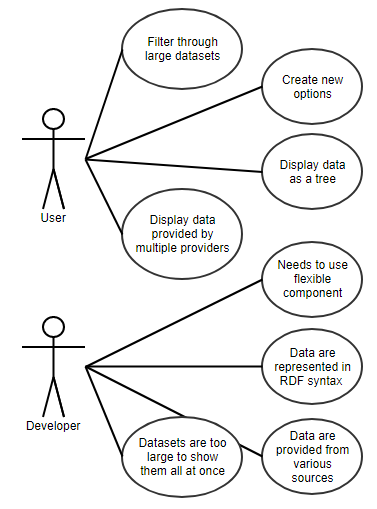
\includegraphics[width=.7\textwidth]{use-case-diagram}
    \decoRule
    \caption[Use Case diagram]{Use Case diagram}
    \label{fig:use-case-diagram}
 \end{figure}

%----------------------------------------------------------------------------------------
%	SECTION 3
%----------------------------------------------------------------------------------------

\section{Providers APIs research}

Firstly, lets quickly introduce what Application  Programming Interface ( API ) is. API stands for Application Programming Interface. It is a program layer that is responsible for interacting with users, giving them responses based on their request. We will be focusing only on Web API. The simplest way to describe Web API is that Web API is set of dedicated web URLs, somewhere on the internet that return some response (usually in text format) to the requestor. There are several types of Web APIs. From historical SOAP (Simple Object Access Protocol) \parencite{soap} and SOA to more modern REST (Representational State Transfer) \parencite{rest}. Because nowadays usage of the REST API is highest, let's focus only on this one type. I will be using Spotify API \parencite{spotify_api} as an example, because of their excellent documentation and variety of their endpoints. All Web APIs have three parts. As you can see below, first is their root address, in this case, it is https://api.spotify.com then following a version, but this is an optional part. Next is an endpoint /artists/{id}/albums; notice a {id} parameter in the URL, this is one way how to send some data to the API. Last part is query parameter. Query parameters are at the end of the URL behind question mark and contain key=value pairs connected with an ampersand. Usually, all query parameters are optional because they have a default value specified on the API side.

\vskip 0.1in

\noindent \colorbox{ltGray}{\parbox{\textwidth}{\textcolor{black!90}{\nolinkurl{https://api.spotify.com/v1/artists/1vCWHaC5f2uS3yhpwWbIA6/albums?market=ES&album_type=single&limit=2}}}}

\vskip 0.2in

Each HTTP \parencite{http} request must also have a header part, where are specified some other information. E.g. Accepted-language or encoding, but most important are Referer and Host.

\begin{figure}[th]
    \centering
    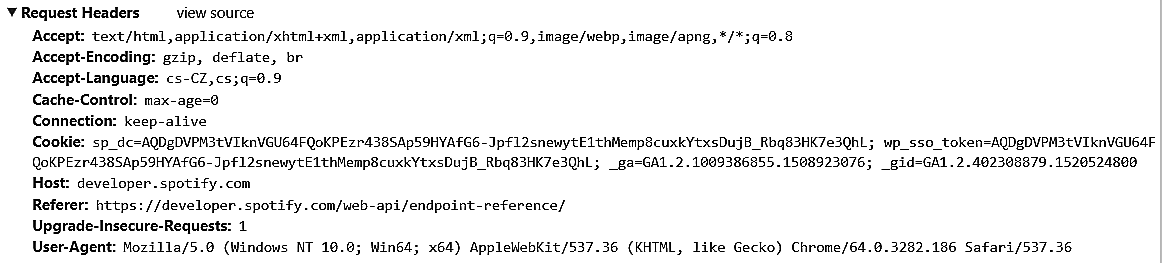
\includegraphics[width=\textwidth]{request_header}
    \decoRule
    \caption[Request header]{Example of request header}
    \label{fig:request_header}
 \end{figure}

Last part of each request is body part. This is the second way how you can send or get some data. But the data format must be in a format that is supported by the server side. The most commonly-used data format is JSON or XML. Often the service supports multiple formats, and the client can request one or the other by including 'json' or 'xml' in the header field 'Accept'.

The functionality of the Web API is much more complicated. The main problem is the complexity; each API can have different behavior based on what data format provides. As I mentioned earlier, most common data formats are JSON or XML. These are both text file formats, but you can also get images, web pages, music file and much more.

There are some examples of the Web APIs that returns different data types.

\begin{itemize}

\item returning json file: https://api.spotify.com/v1/artists/6sFIWsNpZYqfjUpaC gueju 
\item returning web page: https://open.spotify.com/artist/0OdUWJ0sBjDrqHygG UXeCF
\item returning image: https://u.scdn.co/images/pl/default/438f9b65ac4eb48681
351593142daeb070986293
\item returning music file: https://p.scdn.co/mp3-preview/3eb16018c2a700240e9d
fb8817b6f2d041f15eb1?cid=774b29d4f13844c495f206cafdad9c86
\end{itemize}


Some APIs supports filtering in the server side so you can create a requests to get a specific data you want. For example, this API returns 10 artists whose name contains 'tania'
\begin{itemize}
\item \nolinkurl{https://api.spotify.com/v1/search?q=tania%20bowra&type=artist&limit=10}
\end{itemize}

Most of the time API returns only simplified data object, and to get the full information you must request it with for that specific ID.
\begin{itemize}
\item \nolinkurl{https://api.spotify.com/v1/artists/1vCWHaC5f2uS3yhpwWbIA6/albums} 
\end{itemize}
This request return an object with an array of simplified album objects. To get the full detail of the album object another request must be made. 
\begin{itemize}
\item \nolinkurl{https://api.spotify.com/v1/albums/43977e0YlJeMXG77uCCSMX}
\end{itemize}
This request returns a full album detail.

\bigskip

In conclusion, there is a lot of different Web API types. You can distinguish them based on their response format (JSON, XML, img, CSV, etc.), type of their response – some supports filtering results on their side, some return an only limited amount of data, while another may return only header information (e.g., IDs), so you must make another request for each ID to get detailed information. 
So in my component, I will provide an interface through which user can define how to handle communication with specific option provider (Web API)


%----------------------------------------------------------------------------------------
%	SECTION 4
%----------------------------------------------------------------------------------------

\section{Component architecture}

Firstly let's have a look at the high-level view. Structure of the Intelligent Tree Data Management component consists of the three main parts or sub-components. The core sub-component is called Virtualized-tree-select and represent the input field with a drop-down menu. The second one is component representing modal form for creating new options. And the last one exposes some settings to the UI so the user can change the behavior of the component. Both Settings and Modal form sub-components, together with the main component communicate with Redux store, where all necessary data are stored. The third sub-component is independent on the Redux store because all necessary data are passed down as props from the parent component. More about each sub-component will be described in next chapter.

\begin{figure}[th]
    \centering
    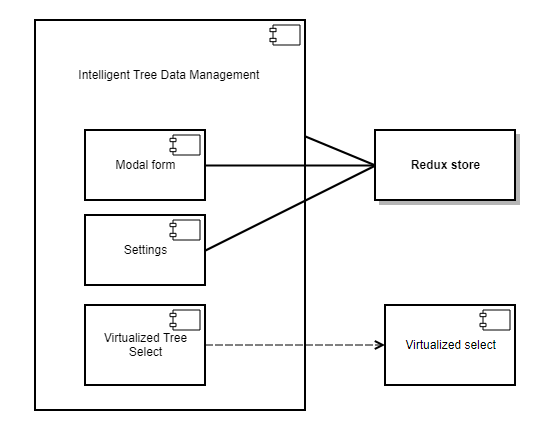
\includegraphics[width=.7\textwidth]{component-diagram}
    \decoRule
    \caption[Architecture]{Component architecture}
    \label{fig:structure}
 \end{figure}

In a low-level point of view, let's look at the UML \parencite{uml} class diagram. As you can see in the image below, main class have three important methods. First method 'onInputChange' check if current input is in history if not, then it call 'getData' for each provider,  and then call 'addNewOptions'. The second method fetches data from providers and returns an array of results. The last method takes the results of the previous call, merge them based on priorities and save it to the already saved options. Other three classes are described in detail in chapter \ref{Chapter5} section 5.2 Component parts. 

The last one is not quite a class, but rather an object of a specific shape. Each option has one or more providers. Provider defines the option characteristics and provides some functions. First function 'response' should return result from the provider. Second one 'toJsonArr' format that response to the array of JSON objects if necessary, and the last one is called only if the label is not a string but array of objects. ( e.g. label: [\{'lang': 'en', 'value': 'This is label'\}, \{'lang':'de', 'value': 'Das ist Label' \}] ). Definition of all properties is in the appendix \ref{AppendixA}.

The association between Provider and Option is 1..N: 1..M because each provider can provide the infinite number of options, but at least it must provide one option. From the other side, it is the same. Each option must have at least one provider. For options that are provided locally the provider called 'local provider' is assigned. 
Next, there is a reflexive association, where each option cant has more than one parent node and N children nodes. Because if you have an option with more than one parent node, then the data cannot be represented as a tree graph.
Last association is between enum class called Type. This class represents the state of the option. Each option can have only one state. However, the state can be contained in N options.

\begin{figure}
    \centering
    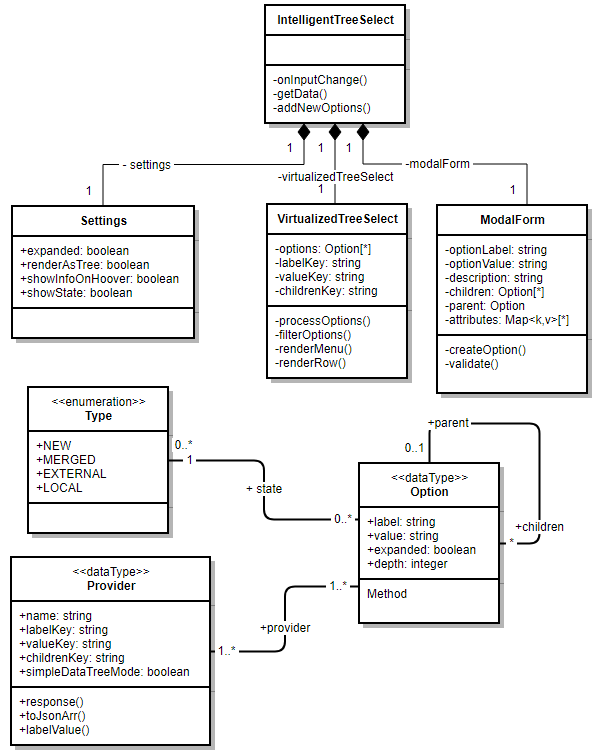
\includegraphics[width=.85\textwidth]{itdm_class_diagram}
    \decoRule
    \caption[Class Diagram]{Component model structure visualized as a class diagram}
    \label{fig:itdm_class_diagram}
 \end{figure}


%----------------------------------------------------------------------------------------
%	SECTION 5
%----------------------------------------------------------------------------------------
\pagebreak

\section{Component life cycle and search cycle}

I will not describe how React handle classes life cycle, because it is not a part of this theses. Also, I will not describe step-by-step of component initialization because it is 
\begin{wrapfigure}{r}{.6\textwidth}
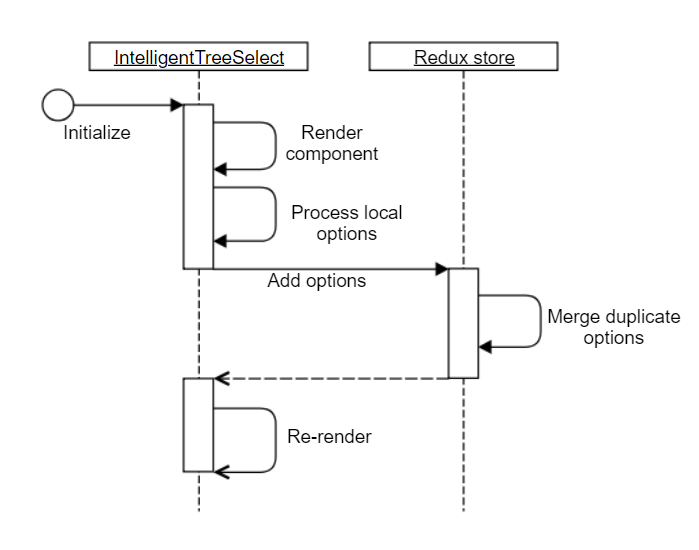
\includegraphics[width=.6\textwidth]{init-sequence-diagram}
    \caption[Initialization]{Component Initialization process}
    \label{fig:init}
\end{wrapfigure}
an out-of-the scope of this thesis. Official React \parencite{react} documentation provides all the necessary information needed. So shortly, as you can see in this image below, the initialization process is divided into three parts. In the first part, the Redux store is created, and all variables (props) are saved. Then the actual HTML elements are rendered and in the last part. If local options are set then they are passed to the virtualized-tree-select sub-component, where they are processed, sorted and the tree graph is created.

\vspace{1cm}

Search cycle is a little bit complicated because some actions are not handled by me, but by the \cite{react-select} and \cite{react-virtualized-select} components. However, I can 
\begin{wrapfigure}{r}{.6\textwidth}
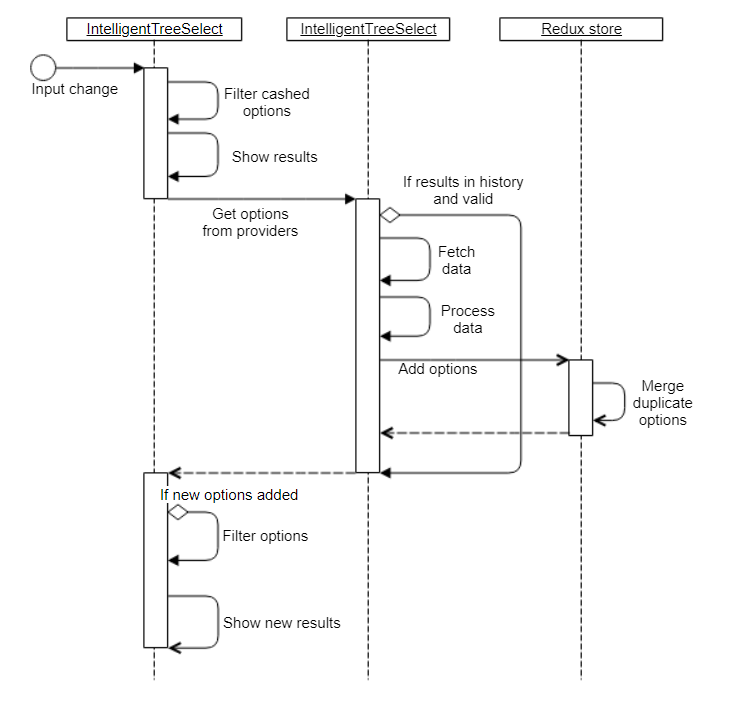
\includegraphics[width=.6\textwidth]{search-sequence-diagram}
    \caption[Search diagram]{Search process}
    \label{fig:search}
\end{wrapfigure}
describe this process from my side. So, when user types into the input field the filter method is triggered by three arguments, current input, already selected options and all local (cashed) options. After that, the results are rendered. Then 'onInputChange' method is executed.The process of that method was already mentioned in the previoud section (4.4 Component architecture) in the second paragraph. This method fetches data from all providers, pre-process them (e.g., convert them to the same format if necessary). Then all new options are saved into the Redux store. Then the 'filterOptions' method is executed again but with new options and finally, new results are displayed. During all of this process, the loading indicator is displayed to the user, so the user is informed that some process is running in the background.


%----------------------------------------------------------------------------------------
%	SECTION 6
%----------------------------------------------------------------------------------------

\section{Creating and adding options}

The process of creating and adding new option is simple. When a user clicks on button 'New option' the modal dialog with Redux form is displayed. Structure of this form is described in chapter \ref{Chapter5} section 5.2.3 Modal form part. After filling up the form and submitting it, the validation function triggers. If the validation finishes with no errors (all required fields are not empty and contains at least 3 characters), the form is submitted. After that, the new option is created and added to all cashed options.

\begin{figure}[h]
	\centering
    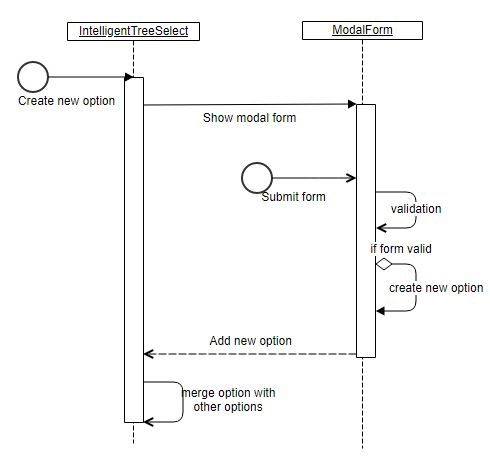
\includegraphics[width=.6\textwidth]{new_option-sequence-diagram}
    \decoRule
    \caption[New option diagram]{Process of creating new option}
    \label{fig:add_new_option}
\end{figure}

%---------------------------------------------------------------------------------------- 
% Chapter Template

\chapter{Implementation} % Main chapter title

\label{Chapter5} % Change X to a consecutive number; for referencing this chapter elsewhere, use \ref{ChapterX}

%----------------------------------------------------------------------------------------
%	SECTION 1
%----------------------------------------------------------------------------------------

\section{Inputs and outputs}

As any other React component you can simply import the main class into your current project and that's pretty much all. Then you can customize the component, provide it some data and start using it. Detailed API is in the appendix, there you can find all properties that you can use. 

The most important property is 'options', this property represents actual options that will be rendered. These options can be represented in two ways. As a graph (simplified version) where each node is represented as one object or as a list of objects (non-simplified) where children are parts of the parent. You can see an example of the options structure in the figure \ref{fig:input-data-example} down below.

Another important property is 'onInputChange', this is a function that will be called when a user selects an option. So this is the way how you can get all selected options. The option that you get back will not be same as you provide. The structure of the new option is following:
\begin{center}
    \begin{longtable}{ | l | l | p{10cm} | }
    \caption{Structure of the returned option} \label{tab:perf} \\
    \hline 
    \multicolumn{1}{|c|}{\textbf{Key name}} & 
    \multicolumn{1}{c|}{\textbf{Type}} & 
    \multicolumn{1}{c|}{\textbf{Description}} \\ \hline 
	\endfirsthead
    \hline 

	provider & Object & object representing provider of that option. See appendix for more detail structure of this object \\ \hline
    state & Object & Object representing state of the option. E.g. \{label: 'Merged', color: 'warning', message: '...'\}, \\ \hline
    expanded & Boolean & Represent if option is expanded (children should be rendered or not)\\ \hline					
    'childrenKey' & List & List of the children IDs. Key name stay same as childrenKey value\\ \hline
    ... &  &  All other properties that was in the original object\\ \hline
    

    \end{longtable}
\end{center}
 

%----------------------------------------------------------------------------------------
%	SECTION 2
%----------------------------------------------------------------------------------------

\section{Component parts}

%----------------------------------------------------------------------------------------
%	SUBSECTION 2.1
%----------------------------------------------------------------------------------------
 \subsection{Virtualized-tree-select part}

Main part virtualized-tree-select component is custom component build on react-virtualized-select and react-select.
This component retains the same API as both components, in addition it provide several new configurations, that configurations can be seen in appendix. So as React-Select, this component generates hidden text input field that contains the value of the
selected option, so it could be submitted as part of the standard form. When the option is selected, ‘onChange’ event is
fired and this event return selected option. All the changes to the select input must be handled by the user; the user
must pass that event value to the ‘value’ attribute of the select component.


%----------------------------------------------------------------------------------------
%	SUBSECTION 2.2
%----------------------------------------------------------------------------------------

\subsection{Settings part}

This is just a collapsible form with several checkboxes that provide some changes to the Virtualized-tree-select
component, like expand or collapse all. Multi-select, this option, if it is checked then the component will provide
multi-selection otherwise only one option will be selectable. Render as a tree, as the name suggests, this option
renders all nodes as a tree also it slightly change filtering because by default if this option is checked the filtering
will also show the whole path in the tree, meaning all parents until root parent will be displayed as well. Display info
on hover, this option enables to show additional information for that node on hover. For example, description.

\begin{figure}[th]
    \centering
    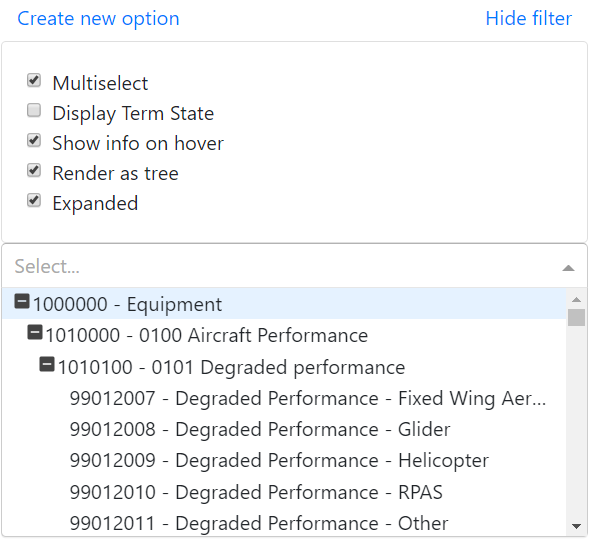
\includegraphics[width=\textwidth]{its-component}
    \decoRule
    \caption[Intelligent tree select component]{Virtualized tree select component with expanded settings}
    \label{fig:its-component}
 \end{figure}

%----------------------------------------------------------------------------------------
%	SUBSECTION 2.3
%----------------------------------------------------------------------------------------
\pagebreak

\subsection{Modal form part}

This component part consists of two dependent react classes. The first one renders empty modal dialog that contains an
only header and close button. The second one renders the actual redux-form in modal body and actions buttons for
submitting or canceling in the modal footer. As I mentioned earlier, this redux-form is used for creating new Nodes. It has several form fields:
\begin{itemize}
    \item Option label (required) – representing a value that is visible in a drop-down box
    \item Option value (required) – representing the unique ID
    \item Option description
    \item Children – a multi-select box containing labels of all other options
    \item Parent – select box containing labels of all other options
\end{itemize}
In the advanced section, there is a button that adds a new pair of form fields. The first one represents object key, second one object value.


After each key press validation is triggered, so the user is informed about invalid inputs before submitting that form. Also, the form is submitted only in the case when all fields are valid. After that new node is created and its added to current tree graph and event ‘onNewOptionCreation’ will be fired.

\begin{figure}[th]
    \centering
    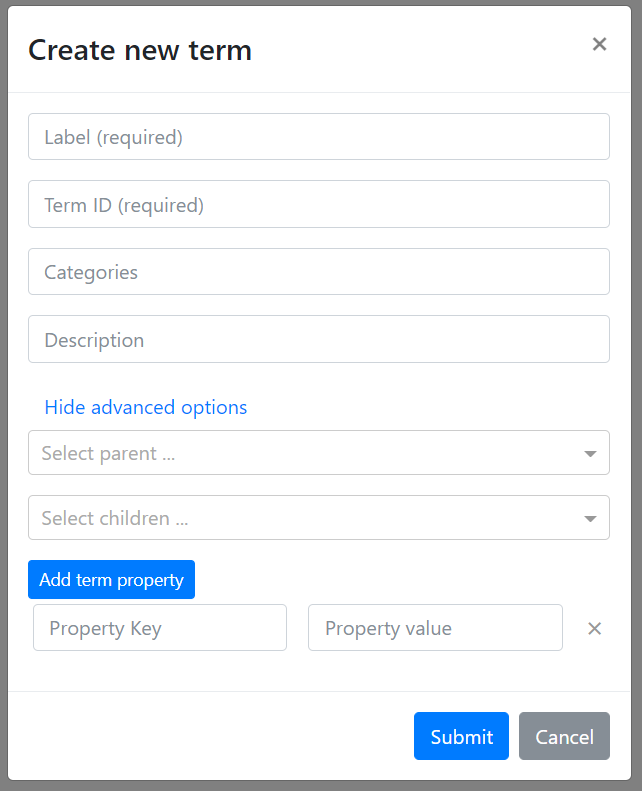
\includegraphics[width=0.7\textwidth]{redux-form}
    \decoRule
    \caption[Redux form]{Redux form for adding new terms}
    \label{fig:redux-form}
 \end{figure}

%----------------------------------------------------------------------------------------
%	SECTION 3
%----------------------------------------------------------------------------------------



%----------------------------------------------------------------------------------------
%	SECTION 4
%----------------------------------------------------------------------------------------

\section{Performance}

Usability of the application may be affected by the performance of the used components. So the performance of my component was one of the critical points during the development. Even that the performance of the current version is acceptable, I still think that there is a space for improvements so that I will continue with the research in this field. As you may know for the flexibility, you have to pay something. Several algorithms have an impact on the overall performance. These algorithms are:

\begin{enumerate}
\item Filter algorithm
\item Algorithm responsible for rendering drop-down menu with options
\item Algorithm that merge all duplicate options
\item Sort algorithm
\item Algorithm for processing data
\end{enumerate}

%----------------------------------------------------------------------------------------
%	SUBSECTION 4.1
%----------------------------------------------------------------------------------------
\section{Render algorithm}

These, who have good experience with HTML, may know that rendering process is a lengthy operation, compared to the JavaScript computation. So I decided to include \cite{react-virtualized-select} that can perfectly handle the problem with rendering a large number of options. The first method is menu rendered and the second one is row renderer. Row renderer is responsible for rendering individual options. Menu renderer renders drop-down menu. This method takes several parameters, most important are - filtered options, currently focused option, option height, drop-down menu height. From these parameters, it can compute how many and what options should be rendered and call row renderer for each of these options. 

The best way is to provide an example. Let's say that filtered options is an array of 20 options. Currently focused option has an index equal to 10. Option height is 20px (pixels) and dropdown height is 100px. So the algorithm renders a container representing dropdown menu with 100px height, then the empty container with a height equal to 400px (20 options times 20px each option) into that previous container. Then algorithm renders individual options with the specified offset, so the method that renders each option is called for the ninth to sixteenth options.

%----------------------------------------------------------------------------------------
%	SUBSECTION 4.2
%----------------------------------------------------------------------------------------
\subsection{Filter algorithm}

The second algorithm that affects performance is an algorithm that filters all options. This algorithm can be divided into three parts. First, all matching options are filtered out. Second, for each filtered option find all parent options (this part will be conditional in future). Last part, all options that are not expanded (their parent have expanded set to false) are also filtered out. 

In detail, the method for filtering options takes 3 arguments. All options, match string and selected options. First of all, options that contain a match string are filtered out. Then the parent options are found for each filtered option. Finding a parent option is done a constant time because the internal data structure of options is same as the structure that is used by Firebase real-time database \parencite{firebase}, which is JSON tree structure. I choose this structure because data are represented as one big JSON object where keys correspond the option value (unique ID of that option) and values of the JSON object are options itself. This structure enables to access the options in constant time. And finally, the algorithm for every option of that previous sub-process (finding parents),  check if an option has a property called 'expanded' equal to 'true', if not then the algorithm removes all children options of that option.

%----------------------------------------------------------------------------------------
%	SUBSECTION 4.3
%----------------------------------------------------------------------------------------
\subsection{Merge algorithm}

Next algorithm merges all duplicate options based on the provider's priority. This algorithm is executed only when new options are added. So if you decided to use only VirtualizedTreeSelect component where you include all options directly this algorithm is never executed. Anyway, this algorithm for each new option checks if that option is already present in the array of all cashed options. If no, then simply adds it and if yes then updates it.

%----------------------------------------------------------------------------------------
%	SUBSECTION 4.4
%----------------------------------------------------------------------------------------
\subsection{Sort algorithm}

Sort algorithm is included in the method that processes all input data. Like the previous algorithm, this algorithm is executed when new options are added. This process takes the option and adds some keys that are used, e.g., parent ID, expanded, state and depth. This algorithm has the same approach like a depth-first search algorithm \parencite{dfs}. So the first item in that sorted array is a root node, next item is left children node of that node and so on, and the last item in last right leaf node.


%----------------------------------------------------------------------------------------
%	SUBSECTION 4.5
%----------------------------------------------------------------------------------------
\subsection{Performance results}

Now let's look at some numbers and data. In this table below you can see how long does is to take for each process to finish. 
For the test purpose, I have one large dataset of 2617 options represented as a graph (simplified) \ref{fig:simplified-data-example} and one smaller dataset of 480 options represented as an array of objects with children as their properties (non-simplified) \ref{fig:non-simplified-data-example}. 

These datasets represented types of aviation accidents and were provided by the \groupname (KBSS). Usage of these datasets is in the INBAS (https://www.inbas.cz/reporting-tool) project. Actual test data will be provided together with the source code.

\begin{figure}
  \centering
  \begin{subfigure}{.5\textwidth}
    \centering
    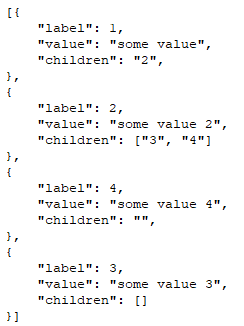
\includegraphics[width=\textwidth]{simplified-data-example}
    \caption[Simplified dataset]{Example of simplified data structure}
    \label{fig:simplified-data-example}
  \end{subfigure}%
  \begin{subfigure}{.5\textwidth}
    \centering
    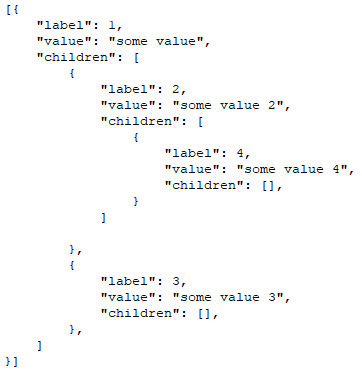
\includegraphics[width=\textwidth]{non-simplified-data-example}
     \caption[Non-Simplified dataset]{Example of non-simplified data structure}
    \label{fig:non-simplified-data-example}
  \end{subfigure}
  \caption[Input data example]{Example of data structure}
  \label{fig:input-data-example}
\end{figure}



This table represents the tests results. Each test was done 10 times on two different test machines and two different web browsers. Data in the table are average values.

\begin{center}
    \begin{longtable}{ | l | l | l | }
    \caption{Time performance based on data structure and data size} \label{tab:perf} \\
    \hline 
    \multicolumn{1}{|c|}{\textbf{Method}} & 
    \multicolumn{1}{c|}{\textbf{Data type}} & 
    \multicolumn{1}{c|}{\textbf{ $\sim$ Time to finish}} 
	\endfirsthead
    
    \hline 
    
    Add new options & simplified & 90 - 200 ms \\ \hline
    Process options & simplified & 4-7 ms \\ \hline
    Filter options & simplified & 1-7 ms \\ \hline
    
    Add new options & non-simplified & 3-5 ms \\ \hline
    Process options & non-simplified & 0-1 ms \\ \hline
    Filter options & non-simplified & 0-1 ms \\ \hline
    Convert dataset & non-simplified & 3-4 ms \\ \hline

    \end{longtable}
\end{center}

Tests were done on two PCs and on the different browsers. However, the differences are negligible (0-2 ms). 
\bigskip

The first test machine specification: Intel i7 series 2.8 Ghz, 16GB ram, win10.
Second test machine specification: AMD FX series 3.5Ghz, 8GB ram, win10. 
Both tests were done on Chrome v66, Firefox v55, and Edge v40 web browsers.

\bigskip
As you can see, even with large datasets (2617 options) all together does not take more than 250 milliseconds. Maybe you think that non-simple datasets are processed faster. That's not really true, because even non-simplified datasets are converted into simplified datasets. That difference between them is because of these data was not so complex. The maximum depth of the child nodes was only 3 compared to the 8 in the other (larger) dataset. So the most significant impact has the complexity of the data, not the type you provide.

%----------------------------------------------------------------------------------------
% Chapter Template

\chapter{Conclusion} % Main chapter title

\label{Chapter6} % Change X to a consecutive number; for referencing this chapter elsewhere, use \ref{ChapterX}

%----------------------------------------------------------------------------------------
%	SECTION 1
%----------------------------------------------------------------------------------------

\section{Future work}

After all, there is still much work that can be done. The current version of the component is in beta version
because there are still some bugs that need to be solved. E.g., problems with destroying react child components
in a drop-down menu or hovering effect. These bugs do not affect the functionality nor visual site, but they are not handled properly and result in errors in console.

Next thing I am planning to look at, as I already mentioned earlier, is a better function for filtering and processing data. Current methods are the first thing that comes to my mind and definitely can be optimized.

Also, I could add more interface features that will make the component even more flexible. 

%----------------------------------------------------------------------------------------
%	SECTION 2
%----------------------------------------------------------------------------------------

\section{Summary}

In conclusion, Intelligent tree select component is based on already great components such as \cite{react-select} and \cite{react-virtualized-select}. This component is providing functionality for displaying options as a tree or creating a new one. As well it can be used with linked data, support two data formats, multiple providers, and much more. A structure is divided into three parts that are independent of themselves. Performance is not perfect in current beta version, but it can perfectly handle a large number of options in acceptable time. Overall compared to other solutions this component is same in core functionality but better in other aspects.

%----------------------------------------------------------------------------------------

%----------------------------------------------------------------------------------------
%	THESIS CONTENT - APPENDICES
%----------------------------------------------------------------------------------------

\appendix % Cue to tell LaTeX that the following "chapters" are Appendices

% Include the appendices of the thesis as separate files from the Appendices folder
% Uncomment the lines as you write the Appendices

% Appendix A

\chapter{Intelligent Tree Select component API} % Main appendix title

\label{AppendixA} % For referencing this appendix elsewhere, use \ref{AppendixA}

All available select props are described here: \url{https://github.com/JedWatson/react-select#select-props} and here: \url{https://github.com/bvaughn/react-virtualized-select/#react-virtualized-select-props}. Additional parameters used by VirtualizedTreeSelect component are described in this table:


\begin{center}
    \begin{longtable}{ | l | l | l | p {6cm} |}
    \caption{Intelligent tree data management component API}\\ \hline
    \multicolumn{1}{|c|}{\textbf{Property}} & 
    \multicolumn{1}{c|}{\textbf{Type}} & 
    \multicolumn{1}{c|}{\textbf{Default value}} & 
    \multicolumn{1}{c|}{\textbf{Description}} \\ \hline 
	\endfirsthead
    \multicolumn{4}{c}%
	{\tablename\ \thetable\ -- \textit{Continued from previous page}} \\
	\hline
	\textbf{Property} & \textbf{Type} & \textbf{Default value} & \textbf{Description} \\
    \endhead
    \multicolumn{4}{r}{\textit{Continued on next page}} \\
	\endfoot
    \hline
	\endlastfoot
    
    childrenKey & PropTypes.string & 'children' & Attribute of option that contains the values (ID) of the children options \\ \hline
    valueKey & PropTypes.string & 'value' & Attribute of option that contains the values of the option \\ \hline
    labelKey & PropTypes.string & 'label' & Attribute of option that contains option label\\ \hline
    labelValue & PropTypes.func & null &  Function that is called only if option[labelKey] is an object not an string. This function get 												option[labelKey] as an parameter and must return a string value. This is useful e.g. if your data are 											multi-language\\ \hline
    
    simpleTreeData & PropTypes.bool & true & Dataset is in simplified format \\ \hline
    expanded & PropTypes.bool & true & Attribute if all options are expanded by default or not \\ \hline
    renderAsTree & PropTypes.bool & true & Attribute if options should be rendered as a tree. If false options are rendered 
    										normally as for default select \\ \hline
    displayInfoOnHover & PropTypes.bool & false & Display tool-tip with additional information \\ \hline      
    displayState & PropTypes.bool & false & Should display state of the option (local, external, new, merged) \\ \hline   
    
    optionRenderer & PropTypes.func & null & Custom way to render options (see below) \\ \hline
    filterOptions & PropTypes.func & null & Custom way to filter options (see below) \\ \hline
    onOptionCreate & PropTypes.func & null & Callback on creating a new option \\ \hline
    
    options & PropTypes.array & [] & Array of default options \\ \hline
    providers & PropTypes.array & [] & Array of provider objects\\ \hline
    
    \end{longtable}
\end{center}

\noindent \textbf{\Large{Provider object structure}}

\begin{center}
\begin{longtable}{ | l | l | l | p {6cm} |}
    \caption{API of the provider object}\\ \hline
    \multicolumn{1}{|c|}{\textbf{Property}} & 
    \multicolumn{1}{c|}{\textbf{Type}} & 
    \multicolumn{1}{c|}{\textbf{Default value}} & 
    \multicolumn{1}{c|}{\textbf{Description}} \\ \hline 
	\endfirsthead
    \multicolumn{4}{c}%
	{\tablename\ \thetable\ -- \textit{Continued from previous page}} \\
	\hline
	\textbf{Property} & \textbf{Type} & \textbf{Default value} & \textbf{Description} \\
    \endhead
    \multicolumn{4}{r}{\textit{Continued on next page}} \\
	\endfoot
    \hline
	\endlastfoot
    
    name & PropTypes.string & (required) & Unique identification of each provider \\ \hline
    response & PropTypes.func & (required) & Function that return data. This function get one string parameter that is equal to current input  \\ 											\hline
    toJsonArr & PropTypes.func & null & Function that is called to convert providers response to JSON array. This function is called only when 											response is not an JSON object \\ \hline

	
    childrenKey & PropTypes.string & 'children' & Attribute of option that contains the values (ID) of the children options \\ \hline
    valueKey & PropTypes.string & 'value' & Attribute of option that contains the values of the option \\ \hline
    labelKey & PropTypes.string & 'label' & Attribute of option that contains option label\\ \hline
    labelValue & PropTypes.func & null &  Function that is called only if option[labelKey] is an object not an string. This function get 												option[labelKey] as an parameter and must return a string value. This is useful e.g. if your data are 											multi-language\\ \hline
    
    simpleTreeData & PropTypes.bool & true & Dataset is in simplified format \\ \hline
    
	\end{longtable}
\end{center}

\pagebreak
\noindent \textbf{\Large{Custom option renderer}}


\begin{center}
    \begin{longtable}{ | l | p {4cm} | p {6cm} |}
    \caption{Option renderer method API}\\ \hline
    \multicolumn{1}{|c|}{\textbf{Property}} & 
    \multicolumn{1}{c|}{\textbf{Type}} & 
    \multicolumn{1}{c|}{\textbf{Description}}
	\endfirsthead
    \multicolumn{3}{c}%
	{\tablename\ \thetable\ -- \textit{Continued from previous page}} \\
	\hline
	\textbf{Property} & \textbf{Type} & \textbf{Description} \\
    \endhead
    \multicolumn{3}{r}{\textit{Continued on next page}} \\
	\endfoot
    \hline
	\endlastfoot
    \hline
    
    focusedOption & PropTypes.object & The option currently-focused in the drop-down. Use this property to determine if your rendered option should be highlighted or styled differently. \\ \hline
    focusedOptionIndex & PropTypes.number & Index of the currently-focused option. \\ \hline
    focusOption	& PropTypes.func & Callback to update the focused option; for example, you may want to call this function on mouse-over. \\ \hline
    labelKey & PropTypes.string & The attribute of option that contains the display text. \\ \hline
    option & PropTypes.object & The option to be rendered. \\ \hline
    options & PropTypes.arrayOf (PropTypes.object) & Array of options (objects) contained in the select menu. \\ \hline
    selectValue & PropTypes.func & Callback to update the selected values; for example, you may want to call this function on click. \\ \hline
    style & PropTypes.object & Styles that must be passed to the rendered option. These styles are specifying the position of each option (required for correct option displaying in the drop-down). \\ \hline
    valueArray & PropTypes.arrayOf (PropTypes.object) & An array of the currently-selected options. Use this property to determine if your rendered option should be highlighted or styled differently. \\ \hline
    valueKey & PropTypes.string & Attribute of option that contains the value. \\ \hline
    onToggleClick & PropTypes.func & Callback to event for clicking on expand button \\ \hline
    childrenKey & PropTypes.string & Attribute of option that contains the values of children options \\ \hline
    
    \end{longtable}
\end{center}


\noindent \textbf{\Large{Custom filter options}}

By default, a component uses a custom function for filtering the options. I don’t recommend overriding this method unless you know what you are doing. For more details, you can look at \url{https://github.com/JedWatson/react-select#advanced-filters}

%----------------------------------------------------------------------------------------
%	BIBLIOGRAPHY
%----------------------------------------------------------------------------------------

\printbibliography[heading=bibintoc]

%----------------------------------------------------------------------------------------

\end{document}  
